\section{Clustering of steady-state correlations in open systems with long-range interactions}

% While the speed of information transfer is always bounded by the speed of light, many quantum platforms operate in a non-relativistic regime where typical velocities are far below this threshold.
% Nevertheless, the  Schr\"odinger equation admits fundamental limits to the rate  at which correlations  can spread throughout the system.
% Such bounds are known as Lieb-Robinson bounds and are connected to a diverse array of phenomena, including the decay of correlations in the ground state \cite{Hastings2006}, generation of topological order \cite{Bravyi2006, Bravyi2010}, efficiency of classical/quantum simulation \cite{Osborne2006,Tran2019a}, hardness of bosonic sampling tasks \cite{Deshpande2018}, heating rates in periodically driven Floquet systems \cite{Abanin2015,Tran2019b}, and signatures of quantum chaos \cite{Lashkari2013,Guo2019}.

To date, most  formulations of Lieb-Robinson bounds apply to closed systems that evolve  via a unitary time-evolution operator.
In such systems, recent advances have proved tight information-transfer bounds for interaction ranges that span the whole spectrum from local \cite{ChenLucas2021graphtheory,WangHazzard2020} to highly non-local regimes \cite{Tran2019a,Chen2019,kuwaharaStrictlyLinearLight2020,Tran2021b}, and have been saturated via explicit state-transfer protocols \cite{Eldredge2017,Tran2020hierarchylinearlightcones,Tran2021}.
While a complete picture for quantum information transfer has emerged for closed quantum systems,  the analogous question for systems that evolve \textit{non-unitarily} in time remains less well understood.
For a broad range of quantum platforms (including noisy quantum simulators), interactions with a  larger environment are unavoidable and must be taken into account to accurately describe dynamics.
While progress in this direction has been made \cite{poulin2010, descamps2013, cubitt2015, Kastoryano2013, Sweke2019}, the question of how the fundamental rate of information transfer differs for systems that interact with some larger environment remains unanswered.

Indeed, the notion of a  Lieb-Robinson bound in an open system may seem \textit{a priori}  surprising from the point of view of quantum trajectories \cite{Knight1998}. In this picture,  in a time-step $dt$ the system's wavefunction either evolves via a non-unitary evolution operator, or a quantum jump discontinuously  alters the state.
A specific  trajectory belonging to a spatially-local Hamiltonian with local dissipation can transfer information faster than  the limit set by the Hamiltonian's Lieb-Robinson bound \cite{Ashida2018}. Intuitively, this is because conditioning on measurements is an inherently nonlocal process.  As an extreme example, it is possible to create a highly-entangled (GHZ) state from a product state in a time $t = \O{1}$ using only locally entangling gates  and measurements, for a specific outcome of the measurements \cite{Pham2013}.  This would violate the Lieb-Robinson bound for local systems, which gives $t = \W{r}$ for distance $r$ \cite{bigO}. After averaging over trajectories, the state of the system can be represented via a density matrix $\rho$ which evolves via a master equation: $ d \rho / dt =  \mL (\rho) $. Subsequently, the notion of a Lieb-Robinson bound is properly restored upon averaging over trajectories.

In this work, we make progress on the question of the fundamental rates of information propagation in open systems by proving a broad class of Lieb-Robinson bounds for systems with long-range interactions---specifically those that decay as a power-law $1/r^\alpha$ in the distance  $r$ between particles, for some $\alpha > 0$.
Such power-law-decaying interactions feature in experimental platforms relevant to quantum computation and simulation, such as Rydberg atoms~\cite{Saffman2010}, trapped ion crystals~\cite{Britton2012,Monroe2021}, polar molecules \cite{Yan2013}, and nitrogen-vacancy color centers in diamond \cite{Yao2012}.
In all of these platforms, interactions with a larger environment cannot be neglected, and a Markovian description of system dynamics is often justified.  In such systems, improved understanding of the fundamental rates of information transfer has spurred the development of optimal protocols for quantum information processing and state transfer \cite{Eldredge2017,Tran2021}.

In addition to bounding dynamics of open long-range systems, we use these Lieb-Robinson bounds to constrain the entanglement structure of the corresponding steady states.
For closed systems, Lieb-Robinson bounds have played an important role in proving rigorous statements on the decay of correlations in gapped ground states \cite{Hastings2006}. This justifies the use of finite-dimensional matrix-product-state representations of the ground state in one-dimensional systems with local interactions \cite{Hastings2007}.
In this work, we prove the clustering of correlations in the steady states of open power-law systems, which may serve as a first step towards establishing an area-law scaling of entanglement for these systems, similar to what was done in Ref.~\cite{Gong2017} for the closed case.

This paper is organized as follows:  in \cref{sec:open-LR}, we summarize the existing Lieb-Robinson bounds for open long-range systems and present two new bounds that are tighter for particular regimes of the power-law exponent $\alpha$.
The first yields a polynomial light cone for $\al > 2d$, using a technique pioneered in Ref.~\cite{Tran2019a}.
The second gives a linear light cone for $\al > 3$ in 1D, using the method from Ref.~\cite{Chen2019}.
In \cref{sec:clustering-of-correlations}, we also prove the clustering of correlations in the steady states of open long-range systems.
Specifically, we provide bounds on the extent of the covariance correlations and mutual information under certain assumptions on the Liouvillian mixing times.
We also prove a stability theorem for the stationary state under local Liouvillian perturbations, generalizing the results of Ref.~\cite{Kastoryano2013}.

\section{Lieb-Robinson bounds for open long-range systems}
\label{sec:open-LR}
In this section, we review the results of the previous best-known Lieb-Robinson bounds for open long-range systems and state two new Lieb-Robinson bounds.

As a general set-up, we consider evolution by a long-range Liouvillian $\L(t)$ that acts on a lattice $\Lambda$ consisting of finite-level systems at each site.
We denote by $\mathcal{H}$ the finite-dimensional Hilbert space representing all possible states of the system and by $\mathcal {B(H)}$ the space of all operators on $\mathcal{H}$.
For an operator $O \in \mathcal {B(H)}$, we will be interested in how its expectation value changes as a function of time: $\langle O(t) \rangle = \tr[ O(t) \rho] = \tr[ O \rho(t)]$, where $\rho$ is the initial state of the system, which evolves (in the Schr\"odinger  picture) via $\rho(t) = e^{\L t} \rho$. For these purposes,
the time-evolution of $O$ can be expressed as $O(t) = e^{\L^\dag t} O$, where $\L^\dag$ is the adjoint Lindblad superoperator, defined as
\begin{align}
	\L^\dag O = +i[H,O] + \sum_i \left[L_i^\dag O L_i - \frac12 \{L_i^\dag L_i,O\}\right],
\end{align}
where $H$ is the Hamiltonian and $L_i$ are Lindblad operators (also referred to as ``jump'' operators) \cite{Breuer2010}.  We emphasize that $O(t)$ is \textit{not} equivalent to the Heisenberg-Langevin time evolution for the operator $O$. For example, if the system has a unique steady state, all operators $O(t)$ will be proportional to the identity at long times: $\lim_{t \rightarrow \infty} O(t) \sim \mathbb{I}$. Thus two operators that do not commute at $t=0$ will start to commute at long times.

We will state the Lieb-Robinson-type bounds in this paper in terms of time-independent Liouvillians. However, we note that the proofs can be generalized with minor modifications to the case of time-dependent Liouvillians---i.e. those for which both $H$ and $L_i$ are allowed to vary in time.

To impose the long-range condition on $\L$, we decompose it into $\L = \sum_{Z\subset \Lambda} \L_Z$, where for any pair of sites $i,j$, we have the condition
\begin{align}
  \label{eq:L-norm-bound}
    \sum_{Z\ni i,j}\|\L_{Z}\|_{\infty} \coloneqq \sup_{O\in\mathcal{B(H)}} \frac{\|\L_{Z}O\|}{\|O\|}\le \frac{1}{\text{dist}(i,j)^\al},
\end{align}
where $\|\cdot\|$ denotes the standard operator norm, or $\infty$-norm, and  $\|\cdot\|_{\infty}$ denotes the superoperator, or ``$\infty \ra \infty$'' norm (referred to as such because the second term in \cref{eq:L-norm-bound} uses the operator $\infty$-norm in both the numerator and the denominator).
Here $\text{dist}(i,j)$ is the distance between $i$ and $j$, and $\al$ is the positive real parameter that controls the long-ranged nature of the interaction.

\subsection{Prior work on open-system Lieb-Robinson bounds}
In Ref.~\cite{Sweke2019}, Sweke \etal~generalized the Lieb-Robinson bound in Ref.~\cite{Hastings2006} for $\al > d$ to open systems.
Letting $A\in \mathcal B(X)$ be an operator supported on $X$, $K_Y\in \mathbb{L}_Y$ be a Liouvillian supported on $Y$, and $e^{\L^\dag t}$ be the evolution under the adjoint Liouvillian superoperator.
The corresponding superoperator bound is:
\begin{align}
  \norm{  K_Y(e^{\L^\dag t}A)} \leq C \|K_Y\|_{\infty} \norm A  \abs{X}\abs{Y}
    \left(
    \frac{e^{vt}-1}{r^{\alpha}}
    \right)
    ,\label{eq:LR-HK-open}
\end{align}
where $r\coloneqq d(X,Y)$, and $C$ and $v$ are $\O1$ constants.
In the closed-system picture, the conventional Lieb-Robinson-type bound can be recovered by choosing $K_Y$ such that $K_Y (O_X) = i[O_X,O_Y]$ and replacing $\|K_Y\|_{\infty}$ with $2\|O_Y\|$.

For this conventional bound, the velocity scales as $v\propto 2^\al $, which diverges in the limit $\al \ra \infty$.
To recover the Lieb-Robinson bound for short-range interacting systems, an improved bound is required that uses a slight modification of the technique from Ref.~\cite{Sweke2019}:
\begin{align}
  \begin{split}
  \norm{  K_Y(e^{\L^\dag t}A)} \leq C \|K_Y\|_{\infty} \norm A  \abs{X}\abs{Y}
    \biggl(&
    \frac{e^{\td vt}}{[(1-\mu)r]^{\alpha}}\\
    &+e^{\td vt-\mu r}
    \biggr),
  \end{split}\label{eq:LR-ZX-open}
\end{align}
where $\mu\in (0,1)$ and $\td v$ are constants, and $\td v$ is independent of $\al$.
The closed-system version of this bound was first proven in Ref.~\cite{Gong2014} for two-body interactions and later generalized to $k$-body interactions in Ref.~\cite{Tran2019b}.
In Ref.~\cite{Sweke2019}, Sweke \etal~also prove Lieb-Robinson-type bounds for $\al \le d$.
For this regime of $\al$, one needs to restrict to a finite-sized lattice, due to the energy being (in general) non-additive for subsystems \cite{Dauxois}.
Denoting the system size of the lattice by $N\coloneqq \abs{\Lambda}$,
the combined strength $J$ of the terms acting on a single site  scales as $J = \Th{N^{1-\al/d}}$ for $\al < d$ and $J = \Th{\log{N}}$ for $\al = d$ \cite{bigO,Guo2019}.
The bound then becomes:
\begin{align}
\label{eq:LR-ZX-open-small-alpha}
    \norm{  K_Y(e^{\L^\dag t}A)} \leq C \|K_Y\|_{\infty} \norm A  \abs{X}\abs{Y}
  \left(
  \frac{e^{J t}-1}{J r^{\alpha}}
  \right).
\end{align}
The effective Lieb-Robinson velocity in this case diverges in the thermodynamic limit, but is finite for all finite $N$.


\subsection{Power-law light-cone bound for $\al > 2d$}
\label{sec:power-law-bound}

We prove a Lieb-Robinson bound  for $\al >2d$ using the truncation-of-unitaries-approach presented by Tran \etal~\cite{Tran2019b}.
The technique takes as input the existing open-systems Lieb-Robinson bound in \cref{eq:LR-ZX-open} and bootstraps it to obtain a tighter bound:
\begin{align}
  \norm{  K_Y(e^{\L^\dag t}A)}
\leq C \|K_Y\|_{\infty}\norm A \frac{t^{\alpha-d}}{r^{\alpha-2d}}.
    \label{eq:LR-Minh-constX}
\end{align}

This bound yields the power-law light-cone contour $t = r^{\frac{\al-2d}{\al-d}}$.
The proof of this bound involves approximating the time evolution of the operators by a sequence of operators that  span successively larger and larger subsets of the lattice, and bounding the error of each successive approximation  by the existing Lieb-Robinson bound.
We provide the full details of the derivation in \cref{sec:minh-bound-proof}.

\subsection{Linear light-cone bound for $d=1$, $\al > 3$}
\label{sec:chen-lucas-bound}
Finally, we prove a bound with a linear light cone for open-long-range systems with $\al > 3$ in $d=1$ dimensions based on the techniques developed in Ref.~\cite{Chen2019}.
In the process, we tighten the tail of the Lieb-Robinson bound given in that work from $1/r$ to approximately $1/r^{\alpha-2}$.
The authors of Ref.~\cite{Chen2019} proved the following bound for the closed-system dynamics of Hamiltonian $H = \sum_{ij} H_{ij}$ consisting of two-body terms:
\begin{align}
\label{eq:chen-lucas-closed-bound}
	\norm{ [e^{iHt} A e^{-iHt},B]} \leq C \norm A \norm{B} \frac{t}{r},
\end{align}
where $B \in \mathcal{B}(Y)$ is an operator supported on $Y$.
Likewise assuming a two-body Liouvillian $\L = \sum_{ij} \L_{ij}$, we obtain the following open-systems bound:
\begin{align}
\label{eq:chen-lucas-open-bound}
	\norm{  K_Y(e^{\L^\dagger t} A)} \leq C \norm{K_Y}_{\infty} \norm A \frac{t}{r^{\alpha-2-o(1)}},
\end{align}
where the $o(1)$ denotes some constant that can be made arbitrarily small.
The result yields a linear light cone $t \gtrsim r$ for all $\al > 3$.
The proof roughly proceeds by expanding out the evolution operator $e^{\L^\dagger t}$ into a series of products of Liouvillian terms $\L_{ij}$.
For each term in the series, we select out a subsequence of terms that move the operator forward (i.e.~towards $Y$) and integrate out the other terms.
By only taking into account the contributions from the terms in the subsequences,  we are able to obtain a tighter Lieb-Robinson bound.
We provide the mathematical details of the proof in \cref{sec:chen-lucas-bound-proof}.

\section{Bounds on correlations in the steady states of open long-range systems}
\label{sec:clustering-of-correlations}
In this section, we prove the clustering of correlations in the steady states of open long-range systems.
We first state a lemma that describes how to use a modified version of the Lieb-Robinson bounds stated in the previous section to bound how far operators can spread under evolution by the (adjoint) Liouvillian $\L^\dagger$.
Specifically, we give a bound on the error of approximating the time-evolution of an operator $A$ supported on a site $X\in\Lam$ by a truncated adjoint Liouvillian that only acts on ball of radius $r$ centered on a site $X\in\Lam$ (see \cref{fig:LRbound_truncated}).

\begin{figure}
\centering
  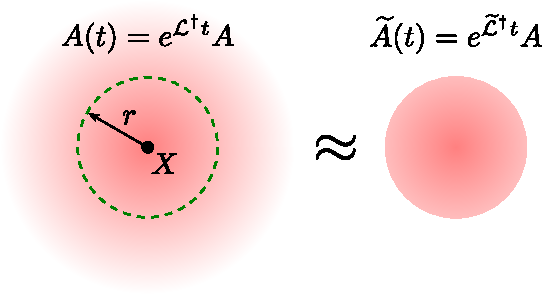
\includegraphics[scale=0.875]{figures/truncate.pdf}
  \caption{The evolution of an operator $A$ initially supported on $X$ by an adjoint Liouvillian $\L^\dag$ can be approximated by the same operator evolved by the truncated version of the Liouvillian, $\td \L^\dag$, supported on a ball of radius $r$ around $X$, up to an error given by $C(r,t)$.}
  \label{fig:LRbound_truncated}
\end{figure}

\begin{lemma}
[Bounds on the error incurred by approximating of time-evolved operators by local ones]
\label{lemma:LRbound_truncated}
    Let $A$ be an operator initially supported on a site $X\in\Lam$ and let $\td \L$ be the restriction of the long-range Liouvillian $\L$ to the ball of radius $r$ centered on $X$.
    Let $\tilde A(t)$ be the time-evolved version of $A$ under $\td \L^\dag$.
    Then the error in the approximation of $A(t)$ by $\tilde A(t)$ is bounded by
    \begin{align}
    \label{eq:LR-bound-approx}
        \|A(t) - \tilde A(t) \| \le K \|A\|\,\mathcal C(r,t),
    \end{align}
    where $K$ is some constant, and $\mathcal C(r,t)$ is a modified version of the standard Lieb-Robinson bound adapted to the problem of locally approximating time-evolved operators.
    In the large-$r$ limit, the tightest-known bounds for open systems with long-range interactions with $\alpha > d$ scale asymptotically as
    \begin{equation}
      \label{eq:LR-bound-cc}
      \ds
      \mathcal C(r,t) \propto \begin{cases} \ds
            e^{vt}/r^{\al-d},& \al > d,
        \\
        \ds t^{\alpha-d+1}/r^{\alpha-3d}
        , & \al > 3d,
        \\ \ds t^2/r^{\alpha-3},& \al > 3, d=1.
      \end{cases}
    \end{equation}
    For $\al \le d$, the bounds also depend on the system size of the lattice $N\coloneqq|\Lam|$.
    When $r \propto N^{1/d}$, the bounds scale as follows:
    \begin{equation}
      \label{eq:LR-bound-cc-small-alpha}
      \mathcal C(N,t) \propto \begin{cases}
        \ds\frac{e^{\Th{N^{1-\al/d}}t}-1}{\Th{N^{1-\al/d}}},& \al < d,
        \\
        \ds\frac{e^{\Th{\log(N)}t}-1}{\Th{\log(N)}},& \al= d.
      \end{cases}
    \end{equation}
    This concludes the statement of \cref{lemma:LRbound_truncated}.
\end{lemma}
The proof of \cref{lemma:LRbound_truncated} follows straightforwardly from the open-system Lieb-Robinson bounds detailed in \cref{sec:open-LR}.
In particular, the three lines of \cref{eq:LR-bound-cc} follow from \cref{eq:LR-ZX-open}, \cref{eq:LR-Minh-constX}, and \cref{eq:chen-lucas-open-bound}, respectively,
while \cref{eq:LR-bound-cc-small-alpha} comes from \cref{eq:LR-ZX-open-small-alpha}.
In \cref{app:sim-local-obs}, we provide the details of the derivation of the bounds in \cref{lemma:LRbound_truncated}.
We now proceed to derive the bounds on clustering of correlations in the steady states of gapped, reversible Liouvillians.

\subsection{Bound on covariance correlations}
In this first section, we show how open-system Lieb-Robinson bounds constrain the correlations in the steady state of a Liouvillian $\L$ with dissipative gap $\lambda$.

The dissipative gap $\lambda >0$
is defined as the magnitude of the least-negative non-zero real part of an eigenvalue of $\L$.
(Throughout this work, we shall also assume that the Liouvillian is \textit{primitive}, i.e.~it has a unique steady state such that $\L$ has one eigenvalue of zero.)
In addition to the Lieb-Robinson bounds,  we will also appeal to certain ``mixing bounds'' which  describe how fast  arbitrary initial states (or various correlation functions) converge to the steady state.

For the mixing bounds, we need to impose ``reversibility'' on the Liouvillian. We say that a Liouvillian $\L$ is $s$-reversible if there exists some operator $\sigma$ such that $\Gamma_s \L^\dag = \L \Gamma_s$ is satisfied;  the superoperator $\Gamma_s$ is defined via $\Gamma_s(f) = ( \sigma^s f \sigma^{1-s} + \sigma^{1-s} f \sigma^s)/2$ and $s \in[0,1]$. For $s$-reversible Liouvillians, it is easy to see that $\sigma$ is the steady state of $\L$ (since $\L^\dag (\mathbb{I}) = 0$).
A sufficient condition for a Liouvillian to satisfy $s$-reversibility (for all $s$) is if the dissipators  $L_i$ satisfy a detailed-balance condition (and the Hamiltonian is zero, $H=0$), which is naturally obeyed for systems coupled to a thermal bath \cite{Kastoryano2013}. (More explicitly, the detailed-balance condition is satisfied if dissipators come in energy raising/lowering pairs with respect to some effective Hamiltonian $\bar{H}$---for example, if $[\bar{H}, L_{\pm}] = \pm \omega L_{\pm}$ and $|L_-| / |L_+| = \exp(2 \beta \omega)$ where $\beta^{-1}$ is an effective temperature.)

Returning to the topic of correlations, we let $\rho$ be a quantum state defined on the lattice $\Lambda$.
We are interested in the \emph{covariance correlation} between non-overlapping $X,Y \in \Lambda$:
\begin{align}
\label{eq:covcorrdef}
  T_\rho (X:Y) := \text{sup}_{\norm{f} = \norm{g} = 1}|\text{Tr}[(f \otimes g)(\rho_{XY} - \rho_X \otimes \rho_Y) ] |,
\end{align}
where $f$ and $g$ are Hermitian operators with $f$ supported on region $X$ and $g$ supported on region $Y$, and where $\rho_{X}$ is the reduced density matrix constructed from $\rho$ by tracing over the complement of $X$. Our goal is to bound this correlation function in terms of $\lam$ and the distance between $X$ and $Y$.

We follow Theorem 9 in Ref.~\cite{Kastoryano2013}.
Let $\sigma$ be the steady state of the Liouvillian.
From the right-hand side of \cref{eq:covcorrdef}, we define
\begin{equation}
\text{Cov}_\sigma(  f, g) \coloneqq \frac{1}{2} \text{Tr}[(f g + g f) \sigma] -\text{Tr}[f \sigma] \text{Tr}[g \sigma],
\end{equation}
which is equivalent to the term inside the sup (because $f$ and $g$ commute).
Now we use the bound (which follows directly from the triangle inequality)
\begin{equation}
\label{eq:covcorr}
  |\text{Cov}_\sigma(f, g)| \leq |\text{Cov}_\sigma (f_t, g_t)| + |\text{Cov}_\sigma(f, g)  - \text{Cov}_\sigma(f_t, g_t)|.
\end{equation}
Here $f_t$ and $g_t$ are the time-evolved versions of $f$ and $g$ under $\L^\dag$.
This step allows us to relate a \textit{static} covariance to  time-dependent quantities;  we will use dynamical bounds to  constrain the form of the latter, then pick an optimal time which maximally bounds the static covariance.

The first term on the right is constrained by the variance bound for $s$-reversible, primitive Liouvillians (see Appendix \ref{sec:var-bound})
\begin{equation} \label{eq:cov-bound}
|\text{Cov}_\sigma (f_t, g_t)| \leq 4 \norm{f} \norm{g}  e^{-2 \lambda t},
\end{equation}
where $\lambda$ is the dissipative gap of $\L$.
Intuitively, this relationship can be understood as follows: the operators $f_t, g_t$  both evolve (in time) toward an operator  that is proportional to the identity, so the covariance between them will eventually tend to zero as a function of time. The rate at which this occurs is set by the dissipative gap of the system.

To bound the second term, we use the relation $\Tr[\sigma f_t]=\Tr[\sigma f]$, which holds for all observables $f$.
This gives:
\begin{align}
& |\text{Cov}_\sigma(f, g)  - \text{Cov}_\sigma(f_t, g_t)| \\
& = \frac12 (|\Tr[(fg-f_tg_t)\sigma] + \Tr[(gf-g_tf_t)\sigma]|) \\
& = \frac12 (|\Tr[((fg)_t-f_tg_t)\sigma] + \Tr[((gf)_t-g_tf_t)\sigma]|) \\
& \leq \frac12 (\|(fg)_t-f_tg_t\|+\|(gf)_t -g_tf_t\|) \\
& \le K \norm{f}  \norm{g} \mathcal{C}(r, t), \label{eq:secondterm}
\end{align}
where $r \coloneqq d(X,Y)$.  We obtain the inequality in the final line using the open-system Lieb-Robinson bounds $\mathcal C(r,t)$ given in \cref{lemma:LRbound_truncated}.
Specifically, we use the following Lemma, which is itself a restatement of Corollary 7 in Ref.~\cite{Kastoryano2013}:
\begin{lemma}
[Time-evolution of spatially separated observables]
  \label{lemma:connectedcorrs}
    Take two operators $A$ and $B$ supported on $X,Y \in \Lam$  respectively such that $r\coloneqq d(X,Y)$, and let $A(t)=e^{\L^\dag t}A$ and $B(t) = e^{\L^\dag t}B$ be their time-evolution under the adjoint Liouvillian $\L^\dag$.
    We also define $(AB)(t) = e^{\L^\dag t}(AB)$.
    Then the following bound holds:
    \begin{align}
    \label{eq:ops-evolving-together}
        \|(AB)(t) - A(t)B(t)\| \le K\|A\|\|B\|\mathcal C(r,t),
    \end{align}
    where $\mathcal C(r,t)$ is given by \cref{lemma:LRbound_truncated} and $K$ is some constant that depends on lattice parameters.
\end{lemma}
\cref{lemma:connectedcorrs} bounds the difference between operators that evolve together in the Heisenberg picture as opposed to evolving separately.
Again we emphasize that $A(t)$, $B(t)$, and $(AB)(t)$ are \textit{not} equivalent to Heisenberg-Langevin evolution, a fact that is at the core of this bound.
We defer the short proof of \cref{lemma:connectedcorrs} to \cref{app:connectedcorrs} and move on to proving the bound on the covariance correlations.

\begin{theorem}[Bounds on steady-state covariance correlations]
\label{theorem:covariancebound}
Consider Hermitian operators $f,g$ which are supported on two non-overlapping subsets $X$ and $Y$ of the $d$-dimensional cubic lattice $\Lambda$, and let $\L$ be an $s$-reversible Liouvillian with stationary state $\sigma$ and dissipative gap $\lambda$ that satisfies the conditions in \cref{eq:L-norm-bound}.
Then there exists a constant $c > 0$ which only depends on $\lambda, v$  such that
\begin{equation}
\label{eq:bounds-covar-correl}
T_\sigma (X:Y) \leq \begin{cases}
     \ds  c \left( r^{\alpha - d} \right)^{\frac{-2 \lambda}{ v + 2\lambda}},& \al > d,
    \\ \ds c \frac{\log(r)^{\al-d+1}}{r^{\al-3d}},& \al > 3d,
    \\ \ds c\frac{\log(r)^2}{r^{\al-3}},& \al> 3, d=1.
    \end{cases}
\end{equation}
\end{theorem}

\begin{proof}
From our previous analysis [see Eqs.~(\ref{eq:cov-bound}) and (\ref{eq:secondterm})] on the covariance correlation in \cref{eq:covcorr}, we have
\begin{equation}
|\text{Cov}_\sigma (f, g)| \leq 4 \norm{f} \norm{g}  \left(e^{-2 \lambda t} + \frac K4 \mathcal{C}(r, t) \right).
\end{equation}
To obtain the tightest bound, we  minimize with respect to $t$ the function
\begin{equation}
\label{eq:cov_corr_minimization}
h(t) =   e^{-\lambda' t} + K' \mathcal{C}(r, t),
\end{equation}
where $\lambda' = 2\lambda, K'= K/4$.

We will perform this minimization exactly for the first case in \cref{eq:bounds-covar-correl}, for which $\mathcal{C}(r,t)$ is given by the first line of \cref{eq:LR-bound-cc}; for the other cases, we instead use an approximation to the optimal ansatz, which allows us to obtain an analytical expression for the bound.
Setting $dh/dt=0$ in \cref{eq:cov_corr_minimization} leads to a minimum at time
\begin{equation}
\bar{t} = -\left( \frac{1}{\lambda'+v} \right) \log \left(  \frac{ K' v }{ \lambda r^{\alpha-d}} \right).
\end{equation}
This implies a minimum:
\begin{align}
h(\bar{t}) &= \left( \frac{K' v}{\lambda' r^{\alpha - d}} \right)^{\frac{\lambda'}{ \lambda' + v}} + \frac{K'}{r^{\alpha - d}}  \left( \frac{K' v} {\lambda' r^{\alpha - d}} \right)^{\frac{-v }{ \lambda' + v }} \nonumber \\
&\leq  c  \left( r^{\alpha - d} \right)^{\frac{-2 \lambda}{ v + 2\lambda}}
\end{align}
for some constant $c$ which depends on $\lambda, v, K$.
Taking the supremum over $f,g$ gives the bound on $T_\sigma (X:Y) $ for $\alpha > d$ in the first line of Eq.~(\ref{eq:bounds-covar-correl}).

For the other two cases, we use the ansatz $t^* = 1+\log(r^\beta)$.
Since the bound in the second line of \cref{eq:LR-bound-cc} scales as
$ \mathcal C(r,t) \propto t^{\alpha-d+1}/r^{\alpha-3d}$
for all $t$, we have
\begin{align}
  h(t^*) &= e^{-\lambda(1+\log(r^\beta))} + K \frac{(1+\log(r^\beta))^{\al-d+1}}{r^{\al-3d}}\nonumber \\
  &= \frac{e^{-\lambda}}{ r^{\lambda\beta}}+ K \frac{(\beta\log(r))^{\al-d+1}}{r^{\al-3d}}
  + \O{\frac{\log^{\al-d}(r)}{r^{\al-3d}}}.
\end{align}
We choose $\beta = (\al-3d)/\lambda$, which is positive for $\al>3d$.
This gives the ultimate bound of
\begin{align}
  h(t^*) &=  \frac{e^{-\lambda}+ K  \left( \frac{\alpha -3d}{\lambda} \log r \right)^{\alpha-d+1}}{r^{\alpha - 3d}} + \O{\frac{\log^{\al-d}(r)}{r^{\al-3d}}}\nonumber\\
  &=
   K\left(\frac{\al-3d}{\lambda}\right)^{\al-d+1}\frac{\log^{\al-d+1}(r)}{r^{\al-3d}} \nonumber\\&\quad \qquad + \O{\frac{\log^{\al-d}(r)}{r^{\al-3d}}},
\end{align}
which proves the second line of Eq.~(\ref{eq:bounds-covar-correl}). For the $d=1$ case in the last line of Eq.~(\ref{eq:bounds-covar-correl}), the argument proceeds similarly, but we obtain a slightly better scaling in the logarithmic factor.
\end{proof}

Here we discuss the scaling of the bounds in \cref{eq:bounds-covar-correl}, which is depicted in \cref{fig:light-cone-scalings}.
The effective exponent of the $1/r$-scaling of the bound for $\al > d$ is $ \al' \equiv (\alpha - d)\frac{2\lambda}{ v + 2\lambda}$, as compared to $\tilde \al \equiv \al-3$ for $\al > 3d$ (neglecting terms doubly logarithmic in $r$).
Since $\al'$ decreases as a function of $v$, the former bound becomes looser for larger $v$.
In more detail, if we let $x = \frac v\lambda$, then $\al' < \tilde \al$ for all $\al > \frac{(3x+4)d}{x}$.
In the limit of $x\ra \infty$, $\tilde \al$ is tighter for all $\al > 3d$.
Thus, for large enough $\al$ and $v$, the power-law light-cone bounds [second line in Eq.~(\ref{eq:LR-bound-cc}), which in turn comes from Eq.~(\ref{eq:LR-Minh-constX})]  give asymptotically tighter bounds on the clustering of covariance correlations than the logarithmic light-cone bound [first line in Eq.~(\ref{eq:LR-bound-cc}), which in turn comes from Eq.~(\ref{eq:LR-ZX-open})].

\begin{figure}[h]
\centering
\label{fig:model1}
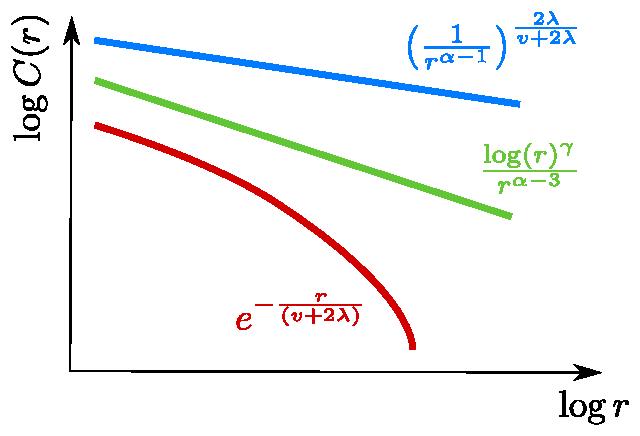
\includegraphics[width=.45\textwidth]{figures/light-cones-log.pdf}
\caption{A log-log plot of the tails of the bounds on the various connected correlation functions in Theorems 1, 2, and 3 for $d = 1$. We include the exponentially decaying tail from the short-range interactions case (red curve) for comparison.
For the power-law decaying bounds, we have different scaling exponents of the power-law tails for the bound for $\alpha >1$ (blue curve) and the bound for $\alpha > 3$ (green curve).
For a given choice of $x = \frac v\lambda$, the relative positioning of the curves
holds for all $\al > \frac{3x+4}{x}$.
In the limit $v \gg \lambda$, the picture holds for all $\al > 3$.}
  \label{fig:light-cone-scalings}
\end{figure}

\subsection{Stability result and mutual information bound}
In this section, we will  use the aforementioned bounds to constrain steady-state properties of open systems with power-law interactions.
In addition to the newly-derived Lieb-Robinson bounds,  we will  appeal to a ``mixing bound'' which provides an upper bound to how fast an arbitrary initial state will converge to the steady state. The following mixing bound was derived in Ref.~\cite{Kastoryano2013d}, and generalizes the mixing bound of classical Markov chains to quantum semigroups:

\begin{lemma}
  \label{cor:mixing}
    Consider a  primitive Liouvillian $\L$ that has a  full-rank steady state  $\sigma$, and is $\frac12$-reversible. Then an arbitrary initial state $\rho$ will converge to $\sigma$ at a rate bounded by
    \begin{equation}
        \lVert \rho(t) - \sigma \lVert_1 \leq \sqrt{2 \log( \lVert \sigma^{-1} \lVert )} e^{-\beta t},
    \end{equation}
    where $\beta$ is called the log-Sobolev constant associated with $\L$.
\end{lemma}
Intuition can be gained by considering an  ``infinite-temperature'' steady state $\sigma = \mathbb{I} /
d_{H}$ where $ d_{H}$ is the dimension of the Hilbert space.  The mixing bound above states that the coefficient in front of the exponential will  scale as $\sqrt{\log(d_{H})}$, i.e.~it will increase with the dimension of the Hilbert space. This is because the convergence toward the unique steady state from an arbitrary initial state can be slow if the dimension of the Hilbert space is large.


\begin{theorem}[Effect of perturbations on reduced steady-state density matrix]
\label{thm:stability_results}
Let $X,Y$ be two non-overlapping subsets of a $d$-dimensional cubic lattice $\Lambda$.  Let $\L_1 $  be a primitive and $\frac12$-reversible Liouvillian with log-Sobolev constant $\beta$, and let $\L_2$ be a Liouvillian perturbation, acting trivially outside of $X$. Let $\rho$ be the stationary state of $\L_1$, and let $\sigma$ be the stationary state of $\L_1  + \L_2$. Then,
\begin{equation}
\label{eq:perturbation_bounds}
\lVert \rho_Y - \sigma_Y  \lVert_1 \leq
\begin{cases}
    \ds c \log (  \lVert \rho^{-1}  \lVert)^{\frac12} \left(\frac1{r^{\alpha - d}} \right)^{\frac{2 \beta}{ v + 2\beta}},& \al > d,
    \\ \ds c \log (  \lVert \rho^{-1}  \lVert)^{\frac12} \frac{\log(r)^{\al-d+1}}{r^{\al-3d}},& \al > 3d,
    \\ \ds c \log (  \lVert \rho^{-1}  \lVert)^{\frac12} \frac{\log(r)^2}{r^{\al-3}},& \hspace{-2em}\al> 3, d=1,
\end{cases}
\end{equation}
where $c$ is a constant and $r$ is the distance between $X$ and $Y$.
\end{theorem}

The theorem basically says that the effects of local perturbations in the Liouvillian will not be felt significantly by the steady state of the system at sufficiently distant locations.
We prove the theorem by first introducing a time-evolved state to interpolate between the two steady states.
This allows us to use a combination of mixing-time and Lieb-Robinson bounds to restrict the terms in this bound.
Then we apply the same minimization procedure used in \cref{theorem:covariancebound} for the covariance-correlations bound to arrive at the stated bounds in \cref{eq:perturbation_bounds} [each of which follow directly from the three cases in \cref{eq:LR-bound-cc}].
We defer the proof of this result, which is similar to the proof of \cref{theorem:covariancebound}, to \cref{app:proof-stability}.

We now prove a bound on the mutual information in the steady state.  The mutual information between two regions $A,B$ is defined as
\begin{equation}
I_\rho(A:B) = S(\rho_{AB} || \rho_A \otimes \rho_B),
\end{equation}
where $S(\rho || \sigma )= \tr[\rho ( \log \rho - \log \sigma)]$ is the relative entropy. The following theorem holds.

\begin{theorem} [Clustering of mutual information]
\label{thm:mutual_information_clustering}
Let $A,B$ be two non-overlapping subsets of a $d$-dimensional cubic lattice $\Lambda$.  Let $\L $  be a primitive and $\frac12$-reversible Liouvillian with log-Sobolev constant $\beta$. Let $\rho$ be the stationary state of $\L$. Then the mutual information between the two regions $I_\rho(A:B)$ is bounded by
\begin{equation}
I_\rho(A:B)  \leq \begin{cases}
       \ds c \log (  \lVert \rho^{-1}  \lVert)^{\frac32} \left( \frac1{r^{\alpha - d}} \right)^{\frac{2 \beta}{ v + 2\beta}},& \al > d,
    \\ \ds  c \log (  \lVert \rho^{-1}  \lVert)^{\frac32} \frac{\log(r)^{\al-d+1}}{r^{\al-3d}},& \al > 3d,
    \\ \ds c\log (  \lVert \rho^{-1}  \lVert)^{\frac32} \frac{\log(r)^2}{r^{\al-3}},& \hspace{-2em}\al> 3, d=1,
    \end{cases}
\end{equation}
where $c$ is a constant and $r$ is the distance between $A,B$.
\end{theorem}

The significance of this result is that the mutual-information correlations in the steady state of an open long-range system decay as a power-law in the distance between regions.
This bound, which relies on the existence of the log-Sobolev constant, is tighter than the naive bound that would result from simply applying the bound on the covariance correlation in \cref{theorem:covariancebound} to $I_\rho(A:B)$.

\begin{proof}

We define the semi-group $\tilde{\L}$ to be the terms in $\L$ that act entirely within balls of radius $r/2$ centered around $A$ and $B$, and let $\sigma$ be the steady state of  $\tilde{\L}$. Simple manipulations imply:
\begin{align}
I_\rho(A:B) &= - S(\rho_{AB})  + S(\rho_A)  + S(\rho_B) \\
& \leq  - S(\rho_{AB})  - \tr[ \rho_A \log \sigma_A ] -  \tr[ \rho_B \log \sigma_B ] \\
&=  S(\rho_{AB} || \sigma_A \otimes \sigma_B).
\end{align}
where we have used $S(\rho || \sigma) \geq 0$ to obtain the inequality.
The RHS further  satisfies the inequality:
\begin{equation}
S(\rho_{AB} || \sigma_A \otimes \sigma_B) \leq \log( ||\rho_{AB}^{-1} ||) || \rho_{AB} - \sigma_A \otimes \sigma_B ||_1,
\end{equation}
which is a standard result (c.f. Eq.~(36) in Ref.~\cite{Kastoryano2013}).
From here, we can apply the bounds in \cref{thm:stability_results}, using $\L_1 = \td \L $, $\L_2 = \L - \td \L$, $Y = A\cup B$, and $X = \Lambda \setminus Y$.
\end{proof}

\section{Summary and outlook}

In this work, we have proven generalized Lieb-Robinson bounds which constrain the dynamics of open, Markovian systems with power-law interactions and used them to constrain correlations in the steady state.

We comment briefly on the tightness of the bounds derived in this work. Intuitively, one might expect that the presence of dissipation should lead to tighter Lieb-Robinson bounds for open systems than for their closed counterparts, since the presence of decoherence from a bath might  limit the speed of quantum information transfer.
In this work, we have  generalized the proof of Lieb-Robinson bounds from closed system dynamics to Markovian evolution (\textit{a priori}, such bounds need not exist for Markovian dynamics).
However, our bounds only depend on interaction range and the dimension of the lattice.
Any bound that only depends on these two inputs cannot be tighter than the corresponding closed-system Lieb-Robinson bound, since the latter is a special case of former.
As such, the saturating protocols for closed systems \cite{Tran2020hierarchylinearlightcones,Tran2021} can be used to saturate open Lieb-Robinson bounds such as those uncovered in  \cref{lemma:LRbound_truncated}.
In the future, it would be interesting to add another degree of freedom into formulations of open Lieb-Robinson bounds: the dissipative gap. (Some progress has been made in showing that Lieb-Robinson velocities can get tighter in dissipative systems \cite{descamps2013}.)
In principle, it might be possible to derive Lieb-Robinson bounds that reduce to closed-system ones when the dissipative gap is zero, and get tighter in the presence of non-zero dissipation.
Then one can develop protocols that saturate the dissipative-gap-dependent bounds.
Another question in this direction is whether the conditional evolution generated via a non-Hermitian Hamiltonian can also exhibit a dissipative-gap-dependent Lieb-Robinson bound that reduces to the conventional one in the dissipationless limit.

Setting aside the idea of a Lieb-Robinson bound that depends on the dissipative gap, there is still the question of generalizing the best-known closed-system bounds to Markovian evolution. In particular, the recent Lieb-Robinson bounds in Refs.~\cite{kuwaharaStrictlyLinearLight2020} and \cite{Tran2021b} both provide opportunities for generalization to open systems.
Such a result would likely require a modification of the interaction-picture technique first developed in \cite{Foss-Feig2015} and used in both subsequent works to open-system dynamics.
Generalizing these bounds would directly lead to tighter bounds on operator spreading in \cref{lemma:LRbound_truncated} and allow us to prove tighter bounds on correlation clustering in steady states (\cref{theorem:covariancebound} and \cref{thm:mutual_information_clustering})

Another way to probe the tightness of the steady-state correlation bounds derived in this work would be to improve the mixing bounds, which currently require the open system to be in thermal equilibrium.
It would be interesting to derive more general mixing bounds which also apply to systems that are out of thermal equilibrium.

One of the salient applications of Lieb-Robinson bounds is in rigorous proofs on the  stability of  the spectral gap in topologically ordered quantum matter. For example, Ref.~\cite{Bravyi2010} used closed-system Lieb-Robinson bounds to  show that spatially local perturbations will not close energy gaps in the toric code, thus leading to phase stability against arbitrary local noise. Can we use a similar approach to show that local perturbations will not close the dissipative gap in a topologically-ordered open system? A robust qubit steady-state structure would be useful toward the quest of passive quantum error correction \cite{Lidar1998}.

Lieb-Robinson bounds can be used  to prove area-law entanglement scaling in the ground state of one-dimensional systems with local interactions \cite{Hastings2007}. This result helps to rigorously justify the validity of the matrix-product state  ansatz for the ground state of such systems.  For closed systems with power-law interactions, Lieb-Robinson bounds can be used to further extend area-law scaling to certain broad classes of systems \cite{Gong2017}. Do the results presented in this paper have similar implications for area-law scaling of the steady state? This would have direct implications for the matrix-product operator ansatz in modeling open systems.

Finally, the Lieb-Robinson-type bounds we proved apply for the operator, or $\infty$-norm.
However, there exists a hierarchy of Lieb-Robinson-like bounds that have the potential to be tighter for certain information processing tasks such as scrambling and transferring a quantum state of a local subsystem without knowledge of the initial state of the rest of the system.
These bounds can use other norms such as the Frobenius norm defined by $\|O\|_F = \sqrt{\Tr{O^\dag O}}$ \cite{Tran2020hierarchylinearlightcones,Kuwahara2020aPolynomialGrowthOutoftimeorder,Yin2020ScramblingAlltoall,Chen2021Frobenius} or apply to free-particle systems \cite{Guo2019,Tran2020hierarchylinearlightcones}.
It would be interesting to generalize these bounds to open systems as well.
